\section{Network Layer}
It is difficult to have a direct path to destination (in ad hoc networks)\\
Routing protocol $\rightarrow$ goal is having a good path from source to destination\\
$\Rightarrow$ good can be:
\begin{itemize}
    \item[$\rightarrow$] the shortest
    \item[$\rightarrow$] the less expensive
    \item[$\rightarrow$] the fastest
\end{itemize}
\subsection{Routing algorithm}
Characteristics:
\begin{itemize}
    \item Graph abstraction for algorithms:
    \begin{itemize}
        \item[$\rightarrow$] Nodes $\rightarrow$ routers
        \item[$\rightarrow$] Edges $\rightarrow$ physical links
    \end{itemize}
    \item Classification:
    \begin{itemize}
        \item[$\rightarrow$] information can be:
        \begin{itemize}
            \item Global $\rightarrow$ all router have complete topology\\
            $\Rightarrow$ Ex: link state algorithm
            \item Decentralised $\rightarrow$ routers know topology only of their neighbours\\
            $\rightarrow$ routing table build when needed $\Rightarrow$ exchange of information\\
            $\Rightarrow$ Ex: Distance vector algorithm
        \end{itemize} 
        \item[$\rightarrow$] algorithm can be:
        \begin{itemize}
            \item Static $\rightarrow$ topology fixed all the time $\rightarrow$ it changes slowly
            \item Dynamic $\rightarrow$ topology changes frequently $\rightarrow$ periodic update of nodes
        \end{itemize}
    \end{itemize}
    \item Example of link state algorithm $\Rightarrow$ Dijkstra algorithm:
    \begin{itemize}
        \item[$\rightarrow$] net topology $\rightarrow$ link costs known to all nodes
        \begin{itemize}
            \item accomplished via link state broadcasting
            \item all nodes have same info
        \end{itemize}
        \item[$\rightarrow$] it computes least cost paths from one node to all the others\\
        $\Rightarrow$ it gives forwarding table for that node
        \item[$\rightarrow$] how it works:\\[0.2cm]
        Notation:
        \begin{itemize}
            \item $c(x,y)$: link cost from node x to y; initially $= + \infty$
            \item $D(v)$: current value of cost of path from source to destination v
            \item $p(v)$: predessor node along path from source to destination v
            \item $N'$: set of node whose least cost path is known
        \end{itemize}
        \newpage
        Algorithm:
        \vspace*{-0.5cm}
        \begin{figure}[!h]
            \centering
            \begin{minipage}{.75\linewidth}
                \begin{algorithm}[H]
                    \captionsetup{labelformat=empty}
                    \begin{algorithmic}[1]
                    \State \textbf{Initialization:}
                    \State $N' = \{u\}$
                    \For {all nodes $v$}
                        \If {$v$ is adjacent to $u$}
                            \State {$D(v) = c(u,v)$}
                        \Else 
                            \State {$D(v) = + \infty$}
                        \EndIf
                    \EndFor
                    \State
                    \State \textbf{Iterations:}
                    \Repeat 
                    \State find $w \notin N' \mid D(w)$ is a minimum
                    \State add $w$ to $N'$
                    \For {\textbf{all} $v$ adjacent to $w$ \& $v \notin N'$}
                        \State $D(v) = min(D(v),$ $D(w) + c(w,v))$ //update $D(v)$
                    \EndFor
                    \Until {all nodes $\in N'$}
                    \end{algorithmic}
                \end{algorithm}
            \end{minipage}
        \end{figure}
    \end{itemize}
\end{itemize}

\subsection{Infrastructure Network vs MANET}
Differences:\\[0.3cm]
\begin{tabular}{|l|l|}
    \hline
    Infrastructure Network & MANET \\
    \begin{minipage}{0.45\linewidth}
        \begin{itemize}
            \item AP/base stations define\\cells/areas
            \item simple routing\\$\rightarrow$ one hop from AP to wireless node
        \end{itemize}
    \end{minipage}
    &
    \begin{minipage}{.45\linewidth}
        \begin{itemize}
            \item no infrastructure\\$\rightarrow$ no static network
            \item hard routing\\$\rightarrow$ some nodes are not close\\$\Rightarrow$ someone must forward data
        \end{itemize}
    \end{minipage}
    \\
    Wired & Wireless \\
    \begin{minipage}{.45\linewidth}
        \begin{itemize}
            \item symmetric link\\$\rightarrow$ bidirectinal
            \item limited redundancy $\rightarrow$ for\\reliability and load sharing
            \item planned links $\rightarrow$ high QoS,\\fixed topology
            \item[]
        \end{itemize}
    \end{minipage}
    &
    \begin{minipage}{.45\linewidth}
        \begin{itemize}
            \item asymmetric link\\$\rightarrow$ unidirectional
            \item random redundancy $\rightarrow$ in\\connectivity between nodes
            \item dynamic links $\rightarrow$ dynamic topology, interference
            \item[]
        \end{itemize}
    \end{minipage}
    \\
    \hline
\end{tabular}
\\[0.3cm]
$\Rightarrow$ Traditional Routing Algorithms $\rightarrow$ doesn't work well for MANET\\
This is because MANETs:
\begin{itemize}
    \item have dynamic topology $\rightarrow$ nodes leave and enter quickly
    \item have minor performance due:
    \begin{itemize}
        \item[$\rightarrow$] energy consumption $\rightarrow$ incompatibility with periodic updates
        \item[$\rightarrow$] limited bandwidth $\rightarrow$ even more to exchange routing info
        \item[$\rightarrow$] asymmetric links $\rightarrow$ info about link + quality of link\\
        $\Rightarrow$ different costs depending on the direction
    \end{itemize}
    \item are innefficient $\rightarrow$ slow convergencee time
    \item are not robust enough
    \item are non-functional $\rightarrow$ large amount of data not dealing with asymmetric links
    \item could have path length (hop count) $\rightarrow$ which may not be the best metric
    \item need routing which rely on data link (not just only network layer updates)\\
    $\rightarrow$ this determines connectivity + quality of links
\end{itemize}
So for a good Unicast Routing Protocol these are all goals:\\[0.3cm]
\begin{minipage}{.5\linewidth}
    \begin{itemize}
        \item minimal control/processing\\overhead
        \item multi-hop path routing
        \item self-starting
        \item energy constraints
        \end{itemize}
\end{minipage}
\begin{minipage}{.5\linewidth}
    \begin{itemize}
        \item traffic patterns $\rightarrow$ inform nodes on what a node is going to do
        \item dynamic topology mantainance
        \item no loops
        \item no central authority
        \end{itemize}
\end{minipage}

\subsection{Routing Procols Classification}
Routing protocols can be classified into 3 different categories:
\begin{itemize}
    \item Proactive (table-driven):
    \begin{itemize}
        \item[$\rightarrow$] routing information always up-to-date
        \item[$\rightarrow$] routing overhead independent of route usage
        \item[$\rightarrow$] used for not so much dynamic networks 
    \end{itemize}
    \item Reactive (Source-initiated):
    \begin{itemize}
        \item[$\rightarrow$] routes maintained only for routes in use $\Rightarrow$ less overhead
        \item[$\rightarrow$] explicit route discovery mechanism
    \end{itemize}
    \item Hybrid
    \begin{itemize}
        \item[$\rightarrow$] combination of proactive and reactive
    \end{itemize}
\end{itemize}

\subsubsection{Proactive Routing Approach}
Characteristics:
\begin{itemize}
    \item based on link-state/distance-vector protocols
    \item each node knows to path to reach another node thanks to consistent tables
    \item there is periodic/event-driven routing updates
    \item routing updates $\Rightarrow$ more overhead
    \item if ad-hoc network is really dynamic $\Rightarrow$ most of updates are not used at all
    \item low latency $\rightarrow$ because route is known
    \item protocols differ on the method to propagate informations\\$\rightarrow$ every node use a unique ID
    \item high route convergence time
    \item Examples: DSDV, WRP \dots
\end{itemize}
Here there are some proactive routing protocols.

\paragraph{Destination Sequenced Distance Vector (DSDV)}\mbox{}\\[0.2cm]
Characteristics:
\begin{itemize}
    \item based on Bellman-Ford algorithm
    \item use sequence number to avoid loops $\rightarrow$ new nodes $\Rightarrow$ higher sequence \mbox{number}
    \item optimizations $\rightarrow$ as incremental data exchange, delayed exchange of updates
    \item packets are transmitted according to routing table
    \item each node:
    \begin{itemize}
        \item[$\rightarrow$] mantains a routing table with entry for each node in the network\\
        $\rightarrow$ <dest\_addr; dest\_seq\_number; next\_hop; hop\_count; install\_time>
        \item[$\rightarrow$] maintains its own sequence number $\Rightarrow$ so it:
        \begin{itemize}
            \item updates if neighbour informations are changed
            \item avoid loops
            \item distinguish new routers
        \end{itemize}
    \end{itemize}
    \item updates:
    \begin{itemize}
        \item[$\rightarrow$] are periodic to keep consistency $\rightarrow$ done with the inclusion of\\<dest\_addr; dest\_seq\_num; hop\_count> $\Rightarrow$ lot of overhead
        \item[$\rightarrow$] nodes send routing tables for important link changes $\rightarrow$ ex: link broken
        \item[$\rightarrow$] if node receive routes from 2 different neighbours $\rightarrow$ it can be chosen:
        \begin{itemize}
            \item the one with higher dest\_seq\_num
            \item the one with lower hop count
        \end{itemize}
        \item[$\rightarrow$] lots of control traffic is created $\rightarrow$ so there are 2 types of routing update
        packets:
        \begin{itemize}
            \item Full dumps:
            \begin{itemize}
                \item ir carries all routing table information
                \item transmitted relatively infrequently
            \end{itemize}
            \item Incremental updates:
            \begin{itemize}
                \item it carries only information changed since last full dump
                \item it fits within one network protocol data unit (NPDU)
                \item when it doesn't fit $\Rightarrow$ full dump
            \end{itemize}
        \end{itemize}
    \end{itemize}
\end{itemize}

\paragraph{Optimized Link State Routing (OLSR)}\mbox{}\\[0.2cm]
Characteristics:
\begin{itemize}
    \item based on state-link algorithm
    \item good for large and dense networks
    \item all links with neighboring Mobile Hosts $\rightarrow$ declared and flooded in entire network
    \item it is done periodic control of messages sent
    \item use of traffic patterns
    \item it minimizes flooding of control traffic using only selected Mobile Hosts\\[0.2cm]
    $\Rightarrow$ Multipoint Relays:
    \begin{itemize}
        \item[$\rightarrow$] it minimizes the flooding of broadcast packets in the network
        \item[$\rightarrow$] each Mobile Host select a set of neighboring Mobile Host to retransmit $\Rightarrow$ reduction of duplicate retransmissions in the same region
        \item[$\rightarrow$] this set can change over time $\rightarrow$ indicated by Hello messages
        \item[$\rightarrow$] tipically are selected neighbour at 1 hop 
    \end{itemize}
\end{itemize}

\paragraph{Clusterhead Gateway Switch Routing (CGSR)}\mbox{}\\[0.2cm]
Characteristics:
\begin{itemize}
    \item nodes organised in hierarchy:
    \begin{itemize}
        \item[$\rightarrow$] Clusterhead $\rightarrow$ selected by election
        \item[$\rightarrow$] Gateway $\rightarrow$ it connects clusterhead
        \item[$\rightarrow$] how it works:
        \begin{enumerate}
            \item Nodes send packet through clusterheads
            \item Clusterheads communicate among themselves using DSDV\\
            $\rightarrow$ two clusters are connected through a gateway node
        \end{enumerate}
    \end{itemize}
\end{itemize}
\subsubsection{Reactive Routing Approach}
Characteristics:
\begin{itemize}
    \item source builds routing on demand by flooding\\$\rightarrow$ nodes receive and broadcast again $\rightarrow$ route discovery cycle
    \item it maintains only active routes
    \item pro $\rightarrow$ less control overhead $\Rightarrow$ better scaling
    \item cons $\rightarrow$ latency or long delay in finding route\\
    RFC\footRFC 3561 not suitable for real-time traffic
    \item route discovery by flooding $\rightarrow$ every node propagates the message\\
    $\Rightarrow$ assumption of algorithms $\rightarrow$ sender need to know the existance of receiver
    \item route mantainance procedure is used to repair routes
    \item Example: AODV, DRS \dots
\end{itemize}

\paragraph{Ad Hoc On-Demand Distance Vector Routing (AODV)}\mbox{}\\[0.2cm]
Characteristics:
\begin{itemize}
    \item RFC 3561 $\rightarrow$ based on DSDV
    \item dest\_seq\_num avoids loops
    \item routing table only exchanges with nodes of a given route
    \item how it finds a route:
    \begin{enumerate}
        \item source sends Route Request Packet (RREQ)\\$\rightarrow$ many routes can be found, but one implemented
        \item nodes floods it to neighbours
        \item Route Reply Packet (RREP) is sent back by destination\\
        $\Rightarrow$ but nodes:
        \begin{itemize}
            \item[$\rightarrow$] respond the first time they receive the request
            \item[$\rightarrow$] reply only if they have contact/valid route with destination
        \end{itemize}
        \item Route Error messages update routes
    \end{enumerate}
    \item if routes are not used $\Rightarrow$ they expire and get discarded
    \begin{itemize}
        \item[$\rightarrow$] it reduces obsolete routes $\Rightarrow$ it doesn't require explicit route maintenance
        \item[$\rightarrow$] it minimizes routes from source to destination
    \end{itemize}
        \item it discovers routes as and when necessary\\$\rightarrow$ path mantained only in involved nodes (routing table)
        \item routes are mantained as long as necessary
        \item nodes have a unique dest\_seq\_num\\$\Rightarrow$ it is increased
        for every change in neighbourhood topology
    \item it utilizes a routing table to store routing informations $\rightarrow$ there are 2 types:
    \begin{itemize}
        \item[$\rightarrow$] for unicast routes $\rightarrow$ path from source to destination
        \item[$\rightarrow$] for multicast routes $\rightarrow$ flooding\\
        $\rightarrow$ it is a problem if a node receives all at once $\Rightarrow$ collision and congestion
    \end{itemize}
    \item route table stores $\rightarrow$ <dest\_add; next\_hop\_add; dest\_seq\_num; life\_time>
    $\rightarrow$ life\_time $\rightarrow$ used as expiring time $\rightarrow$ updated each time route is used
    \item each node maintains list of precursor nodes for each destination to route to\\$\Rightarrow$ help in route mantainance
    \newpage
    \item how route discovery works ($\Rightarrow$ node wishes to send a packet):
    \begin{enumerate}
        \item it checks if destination is in the routing table:
        \begin{itemize}
            \item[$\rightarrow$] Yes $\rightarrow$ it forwards the packet to the next hop;
            \item[$\rightarrow$] No $\rightarrow$ it initiates a route discovery process;
        \end{itemize}
        \item source node creates a new Route Request (RREQ) packet\\
        $\rightarrow$ which contains:
        \begin{itemize}
            \item[$\star$] source\_IP\_add
            \item[$\star$] source\_curr\_seq\_num
            \item[$\star$] dest\_IP\_add
            \item[$\star$] dest\_seq\_num
            \item[$\star$] broad\_ID
        \end{itemize}
        $\rightarrow$ broad\_ID incremented each time a source node uses RREQ
        \\$\rightarrow$ broad\_ID + dest\_IP\_add = unique ID for RREQ
        \item Broadcasting is done via flooding
        \item when intermediate node receives RREQ\\$\Rightarrow$ node sets up
        reverse route entry for source node in its routing table\\
        $\rightarrow$ Reverse Route Entry consists of:
        \begin{itemize}
            \item[$\star$] source\_IP\_add
            \item[$\star$] source\_seq\_num
            \item[$\star$] num\_hops\_to\_source
            \item[$\star$] pred\_IP\_add
            \item[$\star$] life\_time
        \end{itemize}
        $\rightarrow$ nodes can send RREP using reverse route
        \item when RREQ reaches destination $\Rightarrow$ to respond it should have:
        \begin{itemize}
            \item[$\rightarrow$] unexpired entry for destination
            \item[$\rightarrow$] dest\_seq\_num $\geq$ seq\_num\_RREQ (for loop prevention)
        \end{itemize}
        \item there are 2 scenarios depending on satisfaction of conditions in last point. If they are:
        \begin{itemize}
            \item[$\rightarrow$] satisfied $\Rightarrow$ node responds sending a RREP back to source\\
            using unicasting and reverse path
            \item[$\rightarrow$] not satisfied $\Rightarrow$ node increments hop count in RREQ and floods to neighbours
        \end{itemize}
    \end{enumerate}
    Observation\\[0.05cm]
    Also intermediate node can also RREP\\[0.05cm]
    $\rightarrow$ if it knows a more recent path $\Rightarrow$ dest\_seq\_num newer
    \\$\rightarrow$ not used so much $\Rightarrow$ because:
    new RREQ $\Rightarrow$ new dest\_seq\_num\\$\Rightarrow$ intermediate dest\_seq\_num $<$ new dest\_seq\_num
    $\Rightarrow$ it can't send RREP
    \item Timeouts:\\[0.15cm]
    Routing table entry keeping a reverse path is deleted:
    \begin{itemize}
        \item[$\rightarrow$] after a timeout $\Rightarrow$ it should be long enough to allow RREP to come back
        \item[$\rightarrow$] if it is not used for active\_route\_timeout interval\\
        $\rightarrow$ if no data is being sent $\Rightarrow$ that entry will be deleted even if it is valid
    \end{itemize}
    \item Link Failure Detection:
    \begin{itemize}
        \item[$\rightarrow$] neighboring nodes periodically exchange "Hello" messages
        \item[$\rightarrow$] absence of message $\Rightarrow$ link failure
        \item[$\rightarrow$] MAC level ACKs missing $\Rightarrow$ link failure
    \end{itemize}
    \item Optimizations:
    \begin{itemize}
        \item[$\rightarrow$] RREQ are send with a TTL\footTTL with hop count $\Rightarrow$ limit flooding propagation
        \item[$\rightarrow$] initially small TTL $\Rightarrow$ then larger if RREP is not received by source
        \item[$\rightarrow$] Expanding Ring Search:
        \begin{itemize}
            \item it prevents flooding of network during route discovery
            \item it controls TTL of RREQ to search incrementally larger areas
            \item Advantages $\rightarrow$ less overhead when successful
            \item Disadvantages $\rightarrow$ longer delay if route isn't found immediately:
            \begin{itemize}
                \item there could be many possible destinations
                \item it would be better without optimization
                \item maybe it doesn't find the optimal path
            \end{itemize}
        \end{itemize}
    \end{itemize}
\end{itemize}

\paragraph{Dynamic Source Routing (DSR)}\mbox{}\\[0.2cm]
Characteristics:
\begin{itemize}
    \item each data packet has full source route and provokes overhead 
    \item RREQ has attached full source-route and is sent back in RREP
    \item route table overhead is only at source node 
    \item route discovery similar to AODV:
    \begin{enumerate}
        \item sender initiate request
        \item intermediate nodes add their address onto request
        \item when request reaches destination $\Rightarrow$ it includes the full path
    \end{enumerate}
    \item it is better in terms of mobility
\end{itemize}

\newpage

\paragraph{Associativity-Based Routing (ABR)}\mbox{}\\[0.2cm]
Characteristics:
\begin{itemize}
    \item it defines degree of association stability as metric instead of number of hops
    \item nodes with less mobility/better links $\rightarrow$ they have higher stability value
    \item it is DSR-like protocol for routing 
\end{itemize}

\paragraph{Signal Stability Routing (SSR)}\mbox{}\\[0.2cm]
Characteristics:
\begin{itemize}
    \item it defines signal strength of links as metric
    \item RREQ is forwarded only if packet is received over a link with good signal
    \item it is DSR-like protocol for routing
\end{itemize}

\paragraph{Other metrics definition}
\begin{itemize}
    \item Expected Transmission Time (ETT) $\rightarrow$ time to reach a node
    $\Rightarrow$ easy to compute\\$\rightarrow$ more useful than signal strength
    \item Weighted Cumulative Expected Transmission Time (WCETT)\\
    $\rightarrow$ better for multi-radio/asymmetric links
\end{itemize}

\paragraph{Flooding}\mbox{}\\[0.2cm]
Characteristics:
\begin{itemize}
    \item used for Control Packet Delivering
    \item how it works:
    \begin{enumerate}
        \vspace*{-0.05cm}\item sender sends a broadcast packet to all its neighbours $\rightarrow$ to find a route
        \vspace*{-0.05cm}\item neighbours forward it \\$\rightarrow$ if seq\_num no already seen $\Rightarrow$ it avoids packet resending
        \vspace*{-0.05cm}\item destination doesn't forward it \\$\rightarrow$ if destination receives packet $\Rightarrow$ sender can reach the destination
    \end{enumerate}
    \item Pro:
    \begin{itemize}
        \vspace*{-0.05cm}\item[$\rightarrow$] simple and more efficient when there is:
        \begin{itemize}
            \vspace*{-0.05cm}\item high dynamic topology
            \vspace*{-0.05cm}\item small data packet are sent infrequently
        \end{itemize}
        \vspace*{-0.05cm}\item[$\rightarrow$] higher reliability of data delivery $\rightarrow$ multiple paths to reach destination
    \end{itemize}
    \item Cons:
    \begin{itemize}
        \vspace*{-0.05cm}\item[$\rightarrow$] potential high overhead $\rightarrow$ nodes can receive packets multiple times
        \vspace*{-0.05cm}\item[$\rightarrow$] lower reliability of data delivery $\rightarrow$ broadcasting hard to implement\\without overhead increasing
        \vspace*{-0.05cm}\item[$\rightarrow$] potential packet loss $\rightarrow$ more nodes send same packet to same destination simultaneously
    \end{itemize}
\end{itemize}

\subsubsection{DSDV vs AODV}
Differences:
\vspace*{0.2cm}
\begin{center}
    \begin{tabular}{|p{5.5cm}|p{5.5cm}|}
        \hline
        \centering \textbf{DSDV} & \centering \textbf{AODV} \arraybackslash\\
        \begin{minipage}{1 \textwidth}
            \vspace*{0.1cm}
            \begin{itemize}
                \addtolength{\itemindent}{-0.5cm}
                \item every change is broadcasted
                \vspace*{0.15cm}
                \item new neighbours link $\Rightarrow$ news is \newline\hspace*{-0.5cm}broadcasted
                \vspace*{0.15cm}
                \item new broken link $\Rightarrow$ news is \newline\hspace*{-0.5cm}broadcasted
                \vspace*{0.15cm}
                \item more control overhead (high)
                \vspace*{0.15cm}
                \item local movements $\Rightarrow$ global effects
                \item[]
            \end{itemize}
        \end{minipage}
        &
        \begin{minipage}{1 \textwidth}
            \vspace*{0.1cm}
            \begin{itemize}
                \addtolength{\itemindent}{-0.5cm}
                \item no broadcasting necessary 
                \vspace*{0.15cm}
                \item only affected nodes are\newline\hspace*{-0.5cm}informed
                \vspace*{0.15cm}
                \item new broken link $\Rightarrow$ no global \newline\hspace*{-0.5cm}broadcasting
                \vspace*{0.15cm}
                \item less control overhead (low)
                \vspace*{0.15cm}
                \item local movements $\Rightarrow$ local effects
                \item[]
            \end{itemize}
        \end{minipage}
        \\
        \hline
    \end{tabular}
\end{center}

\subsubsection{DSR vs AODV}
Differences:
\vspace*{0.2cm}
\begin{center}
    \begin{tabular}{|p{5.5cm}|p{5.5cm}|}
        \hline
        \centering \textbf{DSDV} & \centering \textbf{AODV} \arraybackslash\\
        \begin{minipage}{1 \textwidth}
            \vspace*{0.1cm}
            \begin{itemize}
                \addtolength{\itemindent}{-0.5cm}
                \item source route in packet headers \newline\hspace*{-0.5cm}$\Rightarrow$ especially for small packets 
                \vspace*{0.15cm}
                \item routing table mantained only \newline\hspace*{-0.5cm}on source
                \vspace*{0.15cm}
                \item lifetime for routes discovery
                \item[]
            \end{itemize}
        \end{minipage}
        &
        \begin{minipage}{1 \textwidth}
            \vspace*{0.1cm}
            \begin{itemize}
                \addtolength{\itemindent}{-0.5cm}
                \item only predecessor on each \newline\hspace*{-0.5cm}packet
                \vspace*{0.15cm}
                \item routing tables mantained also \newline\hspace*{-0.5cm}on nodes
                \vspace*{0.15cm}
                \item no lifetime for routes discovery
                \item[]
            \end{itemize}
        \end{minipage}
        \\
        \hline
    \end{tabular}
\end{center}

\subsubsection{Other Routing Protocols}
There are other protocols:
\begin{itemize}
    \item Hybrid:
    \begin{itemize}
        \item[$\rightarrow$] Zone Routing Protocol (ZRP)
    \end{itemize}
    \item Geographic Routing Protocols:
    \begin{itemize}
        \item[$\rightarrow$] Location Aided Routing (LAR)
        \item[$\rightarrow$] Distance Routing Effect Algorithm for Mobility (DREAM)
        \item[$\rightarrow$] Greedy Perimeter Stateless Routing (GPSR)
    \end{itemize}
\end{itemize}

\paragraph{Greedy Perimeter Stateless Routing (GPSR)}\mbox{}\\[0.2cm]
Characteristics:
\begin{itemize}
    \item nodes know the destination/neighbours location
    \item each node forwards a packet to its neighbor closest to the destination\\
    $\rightarrow$ using some greedy, local optima algorithms
    \item There is a problem $\rightarrow$ the risk of
    local minima ($\Rightarrow$ two nodes keep exchanging the same packet)
    \item if routing holes are found $\Rightarrow$ it uses perimeter routing (right hand rule)\\
    $\rightarrow$ to find local minimum
    \item Right Hand Rule:
    \begin{itemize}
        \item use of first 3 fingers
        \item it works only in 2D topology
        \item how it works:
        \begin{enumerate}
            \item there is an imaginary line from source to destination
            \item the packet is sent to the first node counterclockwise
        \end{enumerate}
    \end{itemize}
\end{itemize}
\begin{figure}[!h]
    \centering
    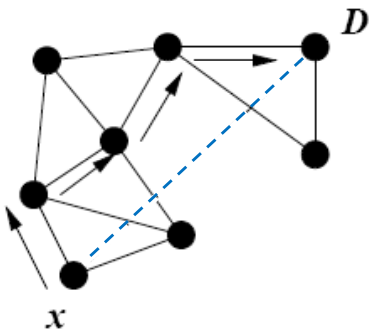
\includegraphics[scale = 0.4]{images/rhr-1.png}
    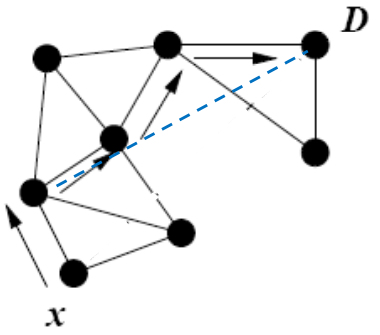
\includegraphics[scale = 0.4]{images/rhr-2.png}
\end{figure}
\begin{figure}[!h]
    \centering
    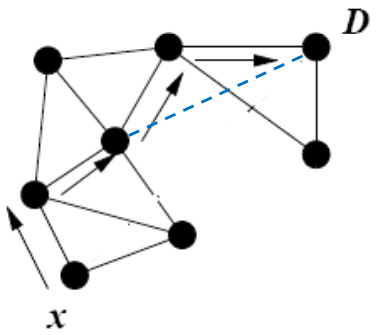
\includegraphics[scale = 0.4]{images/rhr-3.png}
    \caption{Example: Right Hand Rule}
    \label{RightHandRule}
\end{figure}